\begin{figure}[ht]
\centering
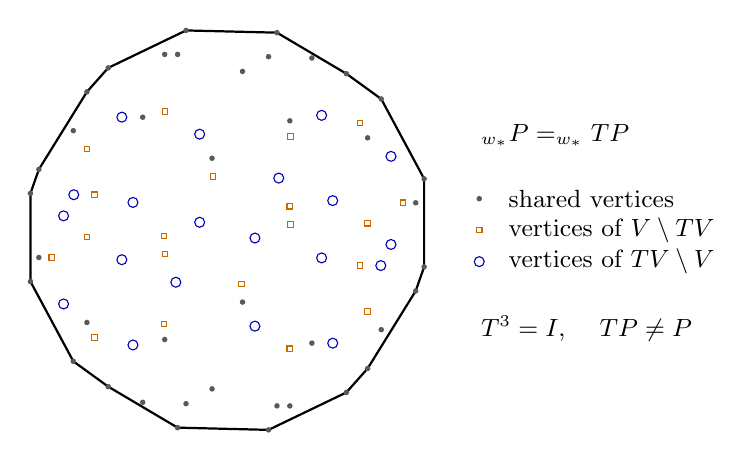
\begin{tikzpicture}[font=\small]
 \draw[thick] (-0.524056,2.536347)--(-1.511992,2.061051)--(-1.782404,1.756843)--(-2.392982,0.771573)--(-2.499929,0.466850)--(-2.499929,-0.652055)--(-1.955447,-1.665540)--(-1.511992,-1.987185)--(-0.631003,-2.508133)--(0.524056,-2.536347)--(1.511992,-2.061051)--(1.782404,-1.756843)--(2.392982,-0.771573)--(2.499929,-0.466850)--(2.499929,0.652055)--(1.955447,1.665540)--(1.511992,1.987185)--(0.631003,2.508133)--cycle;
 \fill[black!65] (0.193468,2.015915) circle (1pt);
 \fill[black!65] (0.193468,-0.913416) circle (1pt);
 \fill[black!65] (-0.794468,2.232139) circle (1pt);
 \fill[black!65] (-0.794468,-1.388712) circle (1pt);
 \fill[black!65] (1.074458,2.186488) circle (1pt);
 \fill[black!65] (1.074458,-1.434364) circle (1pt);
 \fill[black!65] (-1.782404,1.756843) circle (1pt);
 \fill[black!65] (-1.782404,-1.172487) circle (1pt);
 \fill[black!65] (1.955447,1.665540) circle (1pt);
 \fill[black!65] (1.955447,-1.263791) circle (1pt);
 \fill[black!65] (-2.392982,0.771573) circle (1pt);
 \fill[black!65] (-2.392982,-0.347332) circle (1pt);
 \fill[black!65] (-0.524056,2.536347) circle (1pt);
 \fill[black!65] (-0.524056,-2.203410) circle (1pt);
 \fill[black!65] (0.631003,2.508133) circle (1pt);
 \fill[black!65] (0.631003,-2.231624) circle (1pt);
 \fill[black!65] (2.499929,0.652055) circle (1pt);
 \fill[black!65] (2.499929,-0.466850) circle (1pt);
 \fill[black!65] (-1.511992,2.061051) circle (1pt);
 \fill[black!65] (-1.511992,-1.987185) circle (1pt);
 \fill[black!65] (1.511992,1.987185) circle (1pt);
 \fill[black!65] (1.511992,-2.061051) circle (1pt);
 \fill[black!65] (-2.499929,0.466850) circle (1pt);
 \fill[black!65] (-2.499929,-0.652055) circle (1pt);
 \fill[black!65] (-0.631003,2.231624) circle (1pt);
 \fill[black!65] (-0.631003,-2.508133) circle (1pt);
 \fill[black!65] (0.524056,2.203410) circle (1pt);
 \fill[black!65] (0.524056,-2.536347) circle (1pt);
 \fill[black!65] (2.392982,0.347332) circle (1pt);
 \fill[black!65] (2.392982,-0.771573) circle (1pt);
 \fill[black!65] (-1.955447,1.263791) circle (1pt);
 \fill[black!65] (-1.955447,-1.665540) circle (1pt);
 \fill[black!65] (1.782404,1.172487) circle (1pt);
 \fill[black!65] (1.782404,-1.756843) circle (1pt);
 \fill[black!65] (-1.074458,1.434364) circle (1pt);
 \fill[black!65] (-1.074458,-2.186488) circle (1pt);
 \fill[black!65] (0.794468,1.388712) circle (1pt);
 \fill[black!65] (0.794468,-2.232139) circle (1pt);
 \fill[black!65] (-0.193468,0.913416) circle (1pt);
 \fill[black!65] (-0.193468,-2.015915) circle (1pt);
 \draw[orange!80!black] (-0.792831,1.506804) ++(-.035,-.035) rectangle ++(.07,.07);
 \draw[orange!80!black] (-0.182253,0.681648) ++(-.035,-.035) rectangle ++(.07,.07);
 \draw[orange!80!black] (0.804046,1.190759) ++(-.035,-.035) rectangle ++(.07,.07);
 \draw[orange!80!black] (0.804046,0.071855) ++(-.035,-.035) rectangle ++(.07,.07);
 \draw[orange!80!black] (-1.780768,1.031508) ++(-.035,-.035) rectangle ++(.07,.07);
 \draw[orange!80!black] (-0.792831,-0.303622) ++(-.035,-.035) rectangle ++(.07,.07);
 \draw[orange!80!black] (1.685036,1.361332) ++(-.035,-.035) rectangle ++(.07,.07);
 \draw[orange!80!black] (1.685036,-0.449093) ++(-.035,-.035) rectangle ++(.07,.07);
 \draw[orange!80!black] (-1.780768,-0.087397) ++(-.035,-.035) rectangle ++(.07,.07);
 \draw[orange!80!black] (2.229517,0.347848) ++(-.035,-.035) rectangle ++(.07,.07);
 \draw[orange!80!black] (-2.229517,-0.347848) ++(-.035,-.035) rectangle ++(.07,.07);
 \draw[orange!80!black] (1.780768,-1.031508) ++(-.035,-.035) rectangle ++(.07,.07);
 \draw[orange!80!black] (-1.685036,0.449093) ++(-.035,-.035) rectangle ++(.07,.07);
 \draw[orange!80!black] (-1.685036,-1.361332) ++(-.035,-.035) rectangle ++(.07,.07);
 \draw[orange!80!black] (1.780768,0.087397) ++(-.035,-.035) rectangle ++(.07,.07);
 \draw[orange!80!black] (0.792831,-1.506804) ++(-.035,-.035) rectangle ++(.07,.07);
 \draw[orange!80!black] (-0.804046,-0.071855) ++(-.035,-.035) rectangle ++(.07,.07);
 \draw[orange!80!black] (-0.804046,-1.190759) ++(-.035,-.035) rectangle ++(.07,.07);
 \draw[orange!80!black] (0.792831,0.303622) ++(-.035,-.035) rectangle ++(.07,.07);
 \draw[orange!80!black] (0.182253,-0.681648) ++(-.035,-.035) rectangle ++(.07,.07);
 \draw[blue!70!black] (2.079026,-0.181679) circle (1.8pt);
 \draw[blue!70!black] (1.198037,-0.352252) circle (1.8pt);
 \draw[blue!70!black] (-0.351013,0.100069) circle (1.8pt);
 \draw[blue!70!black] (2.079026,0.937226) circle (1.8pt);
 \draw[blue!70!black] (0.653555,0.661232) circle (1.8pt);
 \draw[blue!70!black] (1.198037,1.458174) circle (1.8pt);
 \draw[blue!70!black] (-0.351013,1.218973) circle (1.8pt);
 \draw[blue!70!black] (-1.338949,-0.375228) circle (1.8pt);
 \draw[blue!70!black] (-1.338949,1.435198) circle (1.8pt);
 \draw[blue!70!black] (-1.949527,0.449928) circle (1.8pt);
 \draw[blue!70!black] (1.949527,-0.449928) circle (1.8pt);
 \draw[blue!70!black] (1.338949,-1.435198) circle (1.8pt);
 \draw[blue!70!black] (1.338949,0.375228) circle (1.8pt);
 \draw[blue!70!black] (0.351013,-1.218973) circle (1.8pt);
 \draw[blue!70!black] (-2.079026,-0.937226) circle (1.8pt);
 \draw[blue!70!black] (-1.198037,-1.458174) circle (1.8pt);
 \draw[blue!70!black] (-2.079026,0.181679) circle (1.8pt);
 \draw[blue!70!black] (0.351013,-0.100069) circle (1.8pt);
 \draw[blue!70!black] (-0.653555,-0.661232) circle (1.8pt);
 \draw[blue!70!black] (-1.198037,0.352252) circle (1.8pt);
 \node[anchor=west] at (3.1,1.2) {$\proj_{w_*}P=\proj_{w_*}TP$};
 \fill[black!65] (3.2,.4) circle (1pt);
 \node[anchor=west] at (3.45,.4) {shared vertices};
 \draw[orange!80!black] (3.165,-.035) rectangle ++(.07,.07);
 \node[anchor=west] at (3.45,0) {vertices of $V\setminus TV$};
 \draw[blue!70!black] (3.2,-.4) circle (1.8pt);
 \node[anchor=west] at (3.45,-.4) {vertices of $TV\setminus V$};
 \node[anchor=west] at (3.1,-1.25) {$T^3=I$, $\quad TP\ne P$};
\end{tikzpicture}
\caption{The common eighteen-edge shadow at $w_*$. The nonshared vertices
project inside it. The equality persists on an open set of views, by
Proposition~\ref{prop:coincidence}. Plot coordinates are rounded for display;
the proof uses the exact scalar products, not this drawing.}
\label{fig:hidden}
\end{figure}
